% Chapter 2: 
\chapter{Literature Review}
\label{chap:relatedwork}
\section{Introduction}

This chapter reviews previous studies on readability assessment, Arabic Natural Language Processing, pretrained transformer language models and ordinal regression methods. It follows how readability prediction moved from traditional handcrafted formulas to modern deep learning and transformer based architectures.

The chapter also presents the challenges of Arabic readability, the existing Arabic readability datasets and earlier work built on pretrained language models such as AraBERTv2. It then reviews the ordinal classification and distance aware learning approaches that motivate the methodology of this thesis, together with the pairwise ranking objectives proposed for readability in other languages. Finally, it surveys the systems developed for the BAREC 2025 Shared Task, since they are the most directly comparable prior work.

\section{Readability Assessment}

\subsection{Traditional Readability Formulas}

Early readability assessment research relied mainly on handcrafted statistical formulas designed to estimate text difficulty using shallow linguistic features such as sentence length, word length, and syllable count \cite{dubay2004principles}.
The Flesch Reading Ease (FRE), the Flesch Kincaid Grade Level (FKGL), the SMOG index and the Gunning Fog index are among the most widely used traditional readability formulas. They were first developed for English texts and became popular because they are simple and cheap to compute.

These formulas assume that longer sentences and more complex words mean a text is harder to read. They give fast estimates, but they miss the deeper semantic, syntactic and contextual information that accurate readability prediction needs.

\begin{table}[H]
\centering
\caption{Traditional readability formulas, all originally designed for English.}
\label{tab:traditional_readability}
\renewcommand{\arraystretch}{1.25}
\begin{tabular}{p{4.3cm} c p{6.2cm}}
\toprule
\textbf{Formula} & \textbf{Year} & \textbf{Features used} \\
\midrule
\raggedright Flesch Reading Ease (FRE) & 1948 & Words per sentence and syllables per word; score from 0 to 100, higher is easier \\
\raggedright Gunning Fog Index & 1952 & Sentence complexity and share of words with three or more syllables \\
\raggedright SMOG Index & 1969 & Number of polysyllabic words \\
\raggedright Flesch--Kincaid Grade Level (FKGL) & 1975 & Words per sentence and syllables per word, mapped to a US school grade \\
\bottomrule
\end{tabular}
\end{table}



\begin{figure}[H]
    \centering
    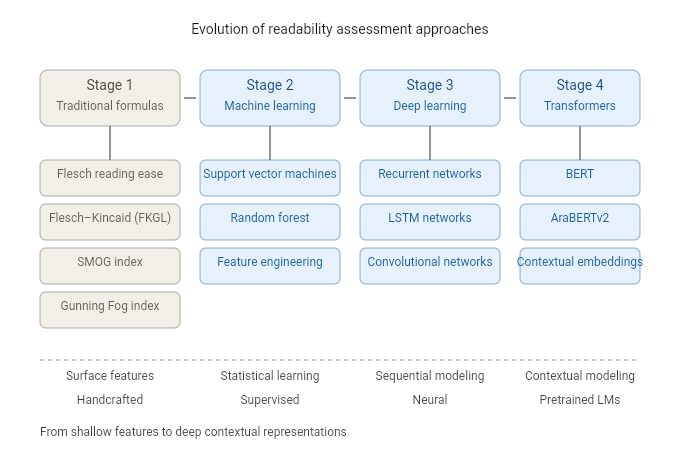
\includegraphics[width=0.98\linewidth]{readability_assessment_evolution@1x.png}
    \caption{How readability assessment evolved, from traditional handcrafted formulas to modern contextual language models based on transformers.}
    \label{fig:evolution}
\end{figure}

\vspace{0.3cm}


Traditional readability formulas are simple and cheap to compute, but they have several important limitations. They rely mostly on shallow handcrafted features and miss semantic meaning, contextual dependencies and linguistic information at the discourse level. These limitations matter even more for morphologically rich languages such as Arabic, where lexical ambiguity and complex word formation patterns make readability prediction considerably harder~\cite{habash2010introduction}.

As research on readability assessment moved forward, machine learning approaches appeared as more powerful alternatives that learn complex linguistic patterns automatically from data. Where traditional handcrafted formulas use a fixed set of shallow features, machine learning methods can exploit a much larger set of lexical, syntactic and statistical features and predict readability more accurately.
\subsection{Machine Learning Approaches}

Machine learning approaches improved considerably on traditional readability formulas, because they learn from data instead of relying only on fixed handcrafted rules. They usually treat readability assessment as a supervised classification or regression problem over manually extracted linguistic features.

Early machine learning systems for readability commonly used lexical, syntactic and statistical features such as sentence length, word frequency, the distribution of parts of speech, the depth of the parse tree and probabilities from language models \cite{schwarm2005reading}.

Several traditional machine learning algorithms have been widely used for readability prediction, including Support Vector Machines (SVM), Random Forests, Logistic Regression, and Naive Bayes classifiers. These models demonstrated improved flexibility and predictive performance compared to traditional readability formulas.

\begin{table}[H]

\centering

\caption{Common machine learning methods used for readability assessment.}

\label{tab:ml_readability}

\begin{tabular}{p{4cm} p{7cm} p{2.5cm}}

\toprule

\textbf{Method} & \textbf{Main Characteristics} & \textbf{Learning Type} \\

\midrule

Support Vector Machines (SVM) & Margin-based supervised classification & Supervised \\

Random Forest & Ensemble decision tree learning & Supervised \\

Logistic Regression & Linear probabilistic classification & Supervised \\

Naive Bayes & Probabilistic feature-based classification & Supervised \\

\bottomrule

\end{tabular}

\end{table}
Notably, the original BAREC benchmark also reports SVM and Decision Tree baselines for Arabic readability: an SVM with a count vectorizer on D3Tok input reaches a QWK of only 56.5\%, and a Decision Tree reaches 52.5\% \cite{elmadani2025barec}. These results confirm that non neural methods are not sufficient for fine grained Arabic readability prediction over 19 levels.
\subsection{Deep Learning Approaches}

Deep learning approaches advanced readability assessment considerably, because they learn hierarchical features automatically from raw text. Traditional machine learning systems depend heavily on handcrafted linguistic features, whereas deep neural networks learn semantic and contextual representations by themselves from large corpora.

Several deep learning architectures have been applied to readability prediction, among them Recurrent Neural Networks (RNN), Long Short Term Memory networks (LSTM) and Convolutional Neural Networks (CNN). These models perform better because they capture sequential dependencies and semantic relations inside the text \cite{martinc2021supervised}.

Recurrent Neural Networks are especially effective at modeling sequential textual information, and LSTM networks learn long range dependencies better thanks to their memory mechanisms. Convolutional Neural Networks have also been applied successfully to readability assessment, where they extract local semantic and syntactic patterns from text representations.

\begin{table}[H]

\centering

\caption{Common deep learning architectures used for readability assessment.}

\label{tab:deep_learning_readability}

\begin{tabular}{p{4cm} p{7cm} p{2.5cm}}

\toprule

\textbf{Architecture} & \textbf{Main Characteristics} & \textbf{Learning Type} \\

\midrule

RNN & Sequential text modeling & Deep Learning \\

LSTM & Long-range dependency modeling & Deep Learning \\

CNN & Local feature extraction and pattern learning & Deep Learning \\

BiLSTM & Bidirectional contextual sequence modeling & Deep Learning \\

\bottomrule

\end{tabular}

\end{table}

Deep learning approaches improved substantially on traditional machine learning methods, but these architectures still had trouble capturing long range contextual dependencies efficiently. Training deep neural networks from scratch also requires large annotated datasets and considerable computational resources.

Transformer based pretrained language models then changed Natural Language Processing, since their self attention mechanisms and their pretraining on large corpora allow them to understand language in context.

\subsection{Transformer-Based Language Models}

Transformer based language models were a major advance in Natural Language Processing, because their self attention mechanisms let them understand language efficiently in context \cite{vaswani2017attention}. Where recurrent neural networks process a sequence step by step, transformer architectures process it in parallel, which lets them model long range dependencies and contextual relations between words more effectively.

One of the most influential transformer models is Bidirectional Encoder Representations from Transformers (BERT), which learns context in both directions to produce deep semantic representations of text \cite{devlin2019bert}. BERT is pretrained on very large text corpora with self supervised objectives such as masked language modeling and next sentence prediction.

Transformer based pretrained language models improved performance considerably on many NLP tasks, among them text classification, sentiment analysis, machine translation, question answering and readability assessment. They capture complex semantic, syntactic and contextual information better than earlier machine learning and deep learning approaches.
\begin{table}[H]

\centering

\caption{Examples of transformer-based language models used in NLP.}

\label{tab:transformer_models}

\begin{tabular}{p{4cm} p{6.5cm} p{2.5cm}}

\toprule

\textbf{Model} & \textbf{Main Characteristics} & \textbf{Language} \\

\midrule

BERT & Bidirectional contextual transformer model & English \\

RoBERTa & Optimized robust BERT pretraining & English \\

DistilBERT & Lightweight compressed transformer model & English \\

AraBERTv2 & Transformer model optimized for Arabic NLP & Arabic \\

\bottomrule

\end{tabular}

\end{table}
Among transformer models, Arabic pretrained language models have attracted growing attention because of the particular linguistic complexity of Arabic. Several Arabic transformer architectures have been proposed to improve Arabic language understanding, and AraBERTv2 performs strongly across many Arabic NLP tasks.

\subsection{AraBERTv2 for Arabic NLP}

AraBERTv2 is a pretrained transformer language model designed specifically for Arabic Natural Language Processing tasks~\cite{antoun2020arabert}. The model uses the BERT architecture (12 layers, 12 attention heads, hidden representations of 768 dimensions) and was pretrained on about 8.6 billion words of Arabic text taken from news articles, Wikipedia and other sources.

What sets AraBERTv2 apart, and the reason we choose it as the backbone in this thesis, is the preprocessing used during pretraining. The original AraBERT was pretrained on plain Arabic text at the word level, while AraBERTv2 was pretrained on text that had first been segmented morphologically with the Farasa segmenter~\cite{darwish2016farasa}. Farasa splits clitics from their host words and marks the boundaries with a \texttt{+} character, which is the same segmentation principle as the D3Tok input representation. When AraBERTv2 receives D3Tok input, the segmented tokens therefore match the distribution it saw during pretraining.

The original BAREC benchmark confirms how much this match matters. Among the four Arabic models tested (AraBERTv02, AraBERTv2, MARBERTv2 and CamelBERT msa), AraBERTv2 was the \emph{only} one whose performance improved with D3Tok input, rising from 76.3\% to 80.0\% QWK on the development set, while the other three models performed the same or worse with D3Tok compared to plain word input \cite{elmadani2025barec}. This empirical result justifies the choice of AraBERTv2 as the fixed backbone in the present work.

\begin{figure}[H]
    \centering
    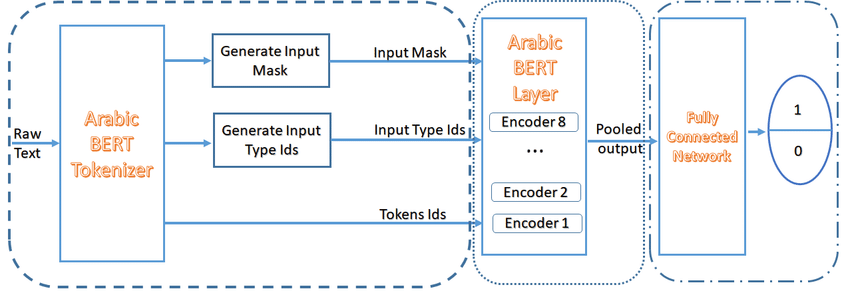
\includegraphics[width=0.79\linewidth]{Arabic-BERT-model-architecture.png}
    \caption{General architecture of transformer-based Arabic language models such as AraBERTv2 for contextual language understanding.}
    \label{fig:arabert_arch}
\end{figure}

\vspace{0.3cm}

Figure~\ref{fig:arabert_arch} shows the general architecture of transformer based Arabic language models. Through its contextual embeddings and self attention mechanisms, AraBERTv2 models the semantic and syntactic relations between Arabic words more effectively than traditional machine learning and earlier deep learning approaches. In readability prediction these contextual representations have a clear advantage over handcrafted features, since they model the semantic complexity and the linguistic dependencies inside the text in more depth.
\subsection{Arabic Readability Datasets}

Building and evaluating automatic readability assessment systems requires annotated datasets of good quality. Compared with English readability research, Arabic readability assessment still has few publicly available benchmark datasets and annotated corpora~\cite{nassiri2023approaches}.

Several Arabic readability datasets and resources have appeared in recent years. The SAMER project produced a leveled readability lexicon for Standard Arabic of about 26,000 lemmas on a scale of five levels \cite{alkhalil2020samer}, which later served as the basis for the SAMER corpus for Arabic text simplification \cite{alhafni2024samer}. DARES provided a readability assessment dataset collected from Saudi school materials \cite{elhaj2024dares}. The OSMAN metric adapted readability scoring to Arabic by taking script specific markers and diacritization into account \cite{elhaj2016osman}. ReadMe++ introduced a multilingual readability benchmark over several domains, whose Arabic split is relevant to Arabic readability research \cite{naous2024readme}. Liberato et al.\ explored strategies for Arabic readability modeling using pretrained models on the SAMER corpus \cite{liberato2024strategies}.

Despite this progress, most existing Arabic readability datasets use coarse scales of only 3 to 5 levels, which limits how finely a model can learn to distinguish between them. This limitation led to a larger and more complete resource, the Balanced Arabic Readability Evaluation Corpus (BAREC), which supports fine grained ordinal readability assessment over 19 ordered levels \cite{elmadani2025barec}.

\subsection{The BAREC Dataset}

The Balanced Arabic Readability Evaluation Corpus (BAREC) was introduced as a large scale benchmark dataset for Arabic readability assessment \cite{elmadani2025barec}. The corpus contains 69,441 Arabic sentences spanning more than one million words, collected from 1,922 documents across three domains (Arts \& Humanities, Social Sciences, and STEM) and three readership groups (Foundational, Advanced, and Specialized).

The main strength of BAREC is its fine grained annotation scheme of 19 ordered readability levels, which follow the Abjad order of the Arabic letters (1-\textit{alif} through 19-\textit{qaf}) and run from kindergarten to postgraduate comprehension. Through the BAREC pyramid the 19 levels can be collapsed into coarser schemes of 7, 5 and 3 levels, so a single model trained at the finest granularity can be evaluated at any coarser one. Six expert Arabic educators annotated the corpus manually, following an adaptation of the Taha Thomure leveling guidelines, and a separate paper describes the annotation protocol in detail \cite{habash2025guidelines}. The reported average pairwise inter-annotator agreement, measured by QWK, is 81.8\%, indicating substantial agreement. The dataset is split at the document level into training (80\%), development (10\%), and test (10\%) sets to prevent data leakage.

\begin{table}[H]

\centering

\caption{Main characteristics of the BAREC dataset.}

\label{tab:barec_characteristics}

\begin{tabular}{p{5cm} p{6cm}}

\toprule

\textbf{Characteristic} & \textbf{Description} \\

\midrule

Language & Modern Standard Arabic \\

Number of Sentences & 69,441 (over 1M words) \\

Documents / Domains & 1,922 documents; 3 domains \\

Readability Levels & 19 ordered levels (collapsible to 7/5/3) \\

Annotation & Manual, by 6 expert Arabic educators \\

Inter-Annotator Agreement & 81.8\% pairwise QWK \\

Target Levels & Kindergarten to postgraduate \\

Data Split & 80\% train / 10\% dev / 10\% test (document-level) \\

\bottomrule

\end{tabular}

\end{table}

The fine grained ordinal structure of BAREC makes it well suited to evaluating ordinal aware learning approaches. Readability levels are ordered by nature, so a prediction error between nearby levels should be penalized less than one between distant levels. The original BAREC benchmark gives the reference results: the best single model (AraBERTv2 + D3Tok + Regression) reaches a test set QWK  of 84.4\%, an average ensemble of six models reaches 84.5\%, and an oracle upper bound that selects the best prediction per sentence reaches 94.7\% \cite{elmadani2025barec}. These figures frame the difficulty of the task and provide the comparison points used in Chapter~4.
\subsection{Ordinal Regression and Distance-Aware Learning}

Ordinal regression is a machine learning paradigm made for prediction tasks whose labels have a natural order \cite{gutierrez2016ordinal}. Where traditional classification treats the classes as unrelated, ordinal prediction takes the relative distance between them into account, which makes it well suited to readability assessment.

In readability prediction the levels are ordered by nature. Predicting level 10 instead of level 11 should count as a smaller error than predicting level 10 instead of level 1. Traditional classification approaches trained with Cross Entropy loss do not model such ordinal relations between labels explicitly.

Several ordinal aware learning methods have been proposed in the literature to address this limitation. They add the ordering of the labels to the training process and penalize distant prediction errors more heavily than nearby ones.
\begin{table}[H]
\centering
\footnotesize
\caption{Loss functions and ordinal heads compared in this thesis.}
\label{tab:ordinal_methods}
\setlength{\tabcolsep}{4pt}
\renewcommand{\arraystretch}{1.2}
\begin{tabular}{L{2.3cm} L{2.4cm} L{4.0cm} L{1.7cm} L{1.8cm}}
\toprule
\textbf{Method} & \textbf{Head and output} & \textbf{Objective} & \textbf{Ordinal / distance} & \textbf{Relation to QWK} \\
\midrule
Cross-Entropy (CE) & Classification, $K$ scores & Log-probability of the gold level & No / No & None \\
Regression (MSE) \cite{elmadani2025barec} & Regression, one score & Squared error between the score and the gold level & Yes / Yes & Loosely coupled \\
CORAL \cite{cao2020coral} & Cumulative, $K{-}1$ logits with one shared projection & Binary cross-entropy summed over the $K{-}1$ thresholds & Yes / Implicit & None \\
CORN \cite{shi2023deep} & Cumulative, $K{-}1$ logits & Binary cross-entropy on $K{-}1$ conditional tasks, each trained on the sentences that reach its level & Yes / Not explicit & None \\
Ordinal Log Loss (OLL) \cite{castagnos2022ordinal} & Classification, $K$ scores & Probability on each wrong level, weighted by its distance from the gold level & Yes / Yes & None \\
Earth Mover's Distance (EMD) \cite{hou2017emd} & Classification, $K$ scores & Squared difference between the predicted and gold cumulative distributions & Yes / Yes & None \\
Soft labels (SOFT) \cite{bertinetto2020soft} & Classification, $K$ scores & Cross-entropy against a target that decays with distance & Yes / Yes & None \\
Soft-QWK \cite{delatorre2018wkl,diaz2019softlabels,trigui2025stbw} & Regression, one score spread over the levels & One minus a differentiable kappa computed over the batch & Yes / Yes & Differentiable surrogate \\
RANK \cite{trokhymovych2024open} & Regression, one score & Squared error plus a margin ranking term on pairs of sentences & Yes / MSE part only & None \\
PLR \cite{lee2022neural} & Regression, one score & Squared error plus a pairwise logistic term on pairs of sentences & Yes / MSE part only & None \\
\bottomrule
\end{tabular}

\vspace{0.15cm}
{\footnotesize Ordinal / distance: whether the objective uses the order of the levels, and whether its penalty grows with the distance from the gold level. $K = 19$ in this thesis.}
\end{table}

Among ordinal-aware approaches, CORAL models ordinal prediction through a sequence of $K{-}1$ ordered binary classification tasks, so that the ordering is encoded in the output structure \cite{cao2020coral}. CORN keeps the $K{-}1$ binary tasks but trains each one as a conditional probability, the probability that a sentence lies above level $k$ given that it lies above level $k-1$; multiplying these conditional probabilities gives cumulative probabilities that can only decrease from one threshold to the next, which keeps the predictions rank-consistent \cite{shi2023deep}. Ordinal log loss extends cross-entropy by weighting the probability given to each wrong level by its distance from the true level \cite{castagnos2022ordinal}. The soft-label loss replaces the one-hot target by a target that decays with distance \cite{bertinetto2020soft}, and the Earth Mover's Distance loss penalises the difference between the predicted and target cumulative distributions \cite{hou2017emd}. The Soft-QWK loss optimises a differentiable surrogate of the QWK metric \cite{delatorre2018wkl,diaz2019softlabels}; because that surrogate is a statistic of the whole batch, it can be lowered by predicting near the mean level, and the STBW system therefore precedes it with a mean squared error warm-up phase \cite{trigui2025stbw}, a design this thesis follows and evaluates in Chapter~\ref{chap:results}.

These methods have demonstrated promising improvements for ordinal prediction tasks across several domains, including medical diagnosis, age estimation, educational assessment, and readability prediction \cite{castagnos2022ordinal}.

\subsection{Pairwise Ranking Objectives for Readability Assessment}
\label{subsec:pairwise_ranking}

A third family of objectives learns readability from comparisons. The model gives every text a single score and is trained on pairs of texts whose relative difficulty is known, so that the harder text of each pair receives the higher score. A pairwise term of this kind uses the order between two texts but not the distance between their levels.

Lee and Vajjala proposed the first neural pairwise ranking model for automatic readability assessment and evaluated it on three English datasets, one French dataset and one Spanish dataset; trained on English alone, it ranked French and Spanish texts with an accuracy above 80\% \cite{lee2022neural}. Trokhymovych et al.\ built an open multilingual system for scoring the readability of Wikipedia articles, together with a dataset in 14 languages that matches Wikipedia articles with their counterparts in simplified Wikipedia and in children's encyclopedias; in a zero-shot setting their model reaches a ranking accuracy above 80\% across the 14 languages \cite{trokhymovych2024open}.

Neither objective has been evaluated in the BAREC benchmark or by the ZAI and STBW systems. This thesis adapts both to 19-level Arabic readability as RANK and PLR, which add a margin ranking term and a pairwise logistic term, respectively, to the mean squared error of the regression head (Chapter~3); both are summarised with the other objectives in Table~\ref{tab:ordinal_methods}.
% NEEDS VERIFICATION (NV2): the margin ranking term of RANK is attributed to Trokhymovych et al. (2024) by the supervisor report; their abstract does not name the training loss. Check the paper's method section.

\section{Systems Developed for the BAREC Shared Task}

The release of the BAREC corpus came with the BAREC 2025 Shared Task on Arabic readability assessment, organized at the Third Arabic Natural Language Processing Conference (ArabicNLP 2025) \cite{elmadani2025sharedtask}. The shared task attracted 22 registered teams from 12 countries, and 17 of them submitted system description papers. It defined two sub tasks, at sentence level and at document level, and three resource tracks, Strict, Constrained and Open, with QWK on a blind test set as the official ranking metric.

The most successful systems combined morphological segmentation (D3Tok) with Arabic pretrained language models, ordinal aware losses and ensembling. Large language models and less standard architectures such as graph neural networks and vision language models generally did worse than the transformer baselines. Only five teams went above the strongest baseline of the organizers (AraBERTv2 + D3Tok + Regression, 84.6\% blind QWK).

Two systems are especially relevant to this thesis. The ZAI system used AraBERTv2 with a CORAL ordinal regression head, trained with a binary cross entropy summed over the $K{-}1$ cumulative thresholds. It selected the checkpoint by QWK, stopped early with a patience of two epochs, and used a single decision threshold tuned on the development set; it reached 85.5\% QWK on the blind test set \cite{nazzal2025zai}. The STBW system used AraBERTv2 with a regression head of a single neuron and a schedule in two phases, a warm up with mean squared error followed by a differentiable Soft QWK objective, which raised its own test QWK from 83.9\% to 84.88\% and reached 85.6\% on the blind test set. Besides the segmented sentence, its input also carries corpus metadata and surface statistics \cite{trigui2025stbw}. These two systems are the reason we include both CORAL and Soft QWK in the present comparison. Their protocols differ, so this thesis reimplements both mechanisms inside one fixed pipeline instead of comparing published numbers.

Table~\ref{tab:barec_systems} summarizes the corpus benchmark, the baselines of the organizers and the participating systems of the shared task, together with their approaches and their QWK scores at sentence level.\footnote{Two systems (ZAI and ANLPers) trained on the development set and are marked with an asterisk; their scores are not strictly comparable.}

\begin{table}[H]
\centering
\footnotesize
\caption{Work on the BAREC dataset: corpus benchmark, organizer baselines, and BAREC 2025 Shared Task systems (sentence-level, Strict track). QWK is the primary metric; higher is better.}
\label{tab:barec_systems}
\begin{tabular}{p{2.4cm} p{0.8cm} p{4.8cm} p{2.2cm} p{1.2cm}}
\toprule
\textbf{Team / Source} & \textbf{Year} & \textbf{Model / Approach} & \textbf{Loss / Method} & \textbf{QWK (\%)} \\
\midrule
\multicolumn{5}{l}{\textit{Corpus benchmark (Elmadani et al., 2025) --- test set}} \\
\midrule
BAREC best single & 2025 & AraBERTv2 + D3Tok & Regression (MSE) & 84.4 \\
BAREC ensemble & 2025 & Average of 6 AraBERTv2 models & Ensemble & 84.5 \\
BAREC oracle & 2025 & Best-of-6 per sentence & Oracle & 94.7 \\
SVM baseline & 2025 & SVM, count vectorizer, D3Tok & Classification & 56.5 \\
\midrule
\multicolumn{5}{l}{\textit{Organizer baselines --- blind test set}} \\
\midrule
Baseline III & 2025 & AraBERTv2 + D3Tok & Regression & 84.6 \\
Baseline II & 2025 & AraBERTv2 + D3Tok & CE & 81.5 \\
Baseline I & 2025 & AraBERTv02 + Word & CE & 80.5 \\
\midrule
\multicolumn{5}{l}{\textit{Shared Task systems --- blind test set (Strict track, sentence-level)}} \\
\midrule
!MSA & 2025 & Ensemble of 4 Arabic PLMs + LLM augmentation & CE + OLL + MSE + ordinal & \textbf{87.5} \\
AMAR & 2025 & Stacked meta-learner over 7 transformers & Regression + meta-classifier & 86.4 \\
mucAI & 2025 & AraBERTv2 + conformal prediction & CE / EMD / Focal & 85.7 \\
STBW & 2025 & AraBERTv2, two-phase training & MSE $\rightarrow$ Soft-QWK & 85.6 \\
ZAI & 2025 & AraBERTv2 + CORAL ordinal head & CORAL (BCE) & 85.5* \\
Syntaxa & 2025 & AraBERTv2 + dependency-graph GNN & GNN & 84.3 \\
MorphoArabia & 2025 & Morphology-aware regression & Regression & 84.2 \\
MARSAD & 2025 & Specialized AraBERT, two-stage & CE $\rightarrow$ WKL & 84.1 \\
Noor & 2025 & Hybrid transformer + features & PLM + features & 83.1 \\
Phantoms & 2025 & Hybrid BERT + linguistic features & PLM + features & 82.7 \\
Qais & 2025 & Fine-tuned PLM (+ LLM) & Classification & 82.5 \\
LIS & 2025 & Curriculum learning with PLMs & Curriculum & 82.4 \\
SATLab & 2025 & Character/token $n$-grams (non-neural) & ML & 82.3 \\
PalNLP & 2025 & Ordinal regression + $K$-fold ensemble & Ordinal regression & 81.1 \\
GNNinjas & 2025 & Lexicon-enriched graph modeling & GNN & 78.5 \\
ANLPers & 2025 & Neural classifiers on embeddings & Neural classifier & 73.0* \\
Pixel & 2025 & Vision-language rendered-text model & VLM & 66.2 \\
\bottomrule
\end{tabular}

\vspace{0.15cm}
{\footnotesize * Trained on the development set; not strictly comparable to the other systems.}
\end{table}

This thesis has a different objective from the shared task systems. It does not try to maximise leaderboard performance through ensembling, data augmentation or external resources. It isolates the effect of the ordinal head and the loss function on a single fixed AraBERTv2 and D3Tok backbone, with every other component kept at the value the benchmark script sets, which gives a controlled view of how much each ordinal aware mechanism contributes on its own. It also adds objectives that neither the benchmark nor the ZAI and STBW systems evaluate: the CORN head and the two pairwise ranking losses of Section~\ref{subsec:pairwise_ranking}.
\section{Summary}

This chapter reviewed the main lines of research on readability assessment, Arabic Natural Language Processing, transformer based language models and ordinal aware learning methods.

It presented the traditional readability formulas with their limitations, then discussed machine learning and deep learning approaches as more advanced alternatives. It then reviewed transformer based pretrained language models, with particular attention to AraBERTv2, and explained why its pretraining on Farasa segmented text makes it the right backbone for D3Tok input.

The chapter also surveyed the existing Arabic readability datasets, among them the SAMER lexicon, DARES and ReadMe++, together with the OSMAN formula adapted to Arabic, and focused on the BAREC corpus as a large scale benchmark for fine grained ordinal readability assessment, with its published benchmark results. Ordinal regression and distance aware learning methods were reviewed and organised into the configurations compared in this thesis, including the CORAL head and the Soft QWK objective, which the benchmark itself does not evaluate, and the CORN head and the pairwise ranking objectives proposed for readability in other languages, which this thesis adapts as RANK and PLR. Finally, it surveyed the systems of the BAREC 2025 Shared Task and put them in a table, identifying ZAI (CORAL) and STBW (mean squared error followed by Soft QWK) as the most directly comparable prior work.

\textit{The next chapter presents the proposed methodology: the corpus and its splits, the D3Tok input, the encoder and the three prediction heads, the exact form of every loss function, the initialisation of the CORAL cut points, the training protocol with its declared differences from the published script, and the evaluation setup.}
